%--------------------------------------------------------------------------------------------------
%	PREAMBOLO
%---------------------------------------------------------------------------------------------------
\documentclass[a4paper,11pt,twoside,openright]{memoir}
\usepackage[utf8x]{inputenc}
%\usepackage{showframe}
\usepackage{geometry} 
%---------------------------------------------------------------------------------------------------
%	Pacchetti ed impostazioni generali

%%%%%%%%%%%%%%%%%%%%%%%%%%%%%%%%%%%%%%%%%%%%%%%%%%
%
% Per la generazione corretta del 
% pdflatex nome_file.tex
% bibtex nome_file.aux
% pdflatex nome_file.tex
% pdflatex nome_file.tex
%
%%%%%%%%%%%%%%%%%%%%%%%%%%%%%%%%%%%%%%%%%%%%%%%

% formato FRONTE RETRO
%\usepackage{epsfig}

\usepackage{plain}
\usepackage{setspace}

%--------------------------------------------------------------------
%------------------------- C H I A R A  layout ----------------------
% Better page layout for A4 paper, see memoir manual.
\settrimmedsize{297mm}{210mm}{*}
\setlength{\trimtop}{0pt} 
\setlength{\trimedge}{\stockwidth} 
\addtolength{\trimedge}{-\paperwidth} 
\settypeblocksize{634pt}{448.13pt}{*} 
\setulmargins{4cm}{*}{*} 
\setlrmargins{*}{*}{*} 
\setmarginnotes{17pt}{51pt}{\onelineskip} 
\setheadfoot{\onelineskip}{2\onelineskip} 
\setheaderspaces{*}{2\onelineskip}{*} 
\checkandfixthelayout
\setlength{\oddsidemargin}{0.35cm}%
\setlength{\evensidemargin}{-0.35cm}%
%
\frenchspacing
% Font with math support: New Century Schoolbook
\usepackage{fouriernc}
\usepackage[T1]{fontenc}
% Text should be in double or 1.5 line spacing, and font size should be
% chosen to ensure clarity and legibility for the main text and for any
% quotations and footnotes. Margins should allow for eventual hard binding.
%
% Note: This is automatically set by memoir class. Nevertheless \OnehalfSpacing 
% enables double spacing but leaves single spaced for captions for instance. 
\OnehalfSpacing 
%
% Sets numbering division level
\setsecnumdepth{subsection} 
\maxsecnumdepth{subsubsection}
%
\usepackage{float}						%Helps to place figures, tables, etc. 
%\newfloat{algo}{tbp}{loa}[subparagraph*]

\usepackage{calc,soul,fourier}
\makeatletter 
\newlength\dlf@normtxtw 
\setlength\dlf@normtxtw{\textwidth} 
\newsavebox{\feline@chapter} 
\newcommand\feline@chapter@marker[1][4cm]{%
	\sbox\feline@chapter{% 
		\resizebox{!}{#1}{\fboxsep=1pt%
			\colorbox{white}{\color{black}\thechapter}% 
		}}%
		\rotatebox{0}{% 
			\resizebox{%
				\heightof{\usebox{\feline@chapter}}+\depthof{\usebox{\feline@chapter}}}% 
			{!}{\scshape\so\@chapapp}}\quad%
		\raisebox{\depthof{\usebox{\feline@chapter}}}{\usebox{\feline@chapter}}%
} 
\newcommand\feline@chm[1][4cm]{%
	\sbox\feline@chapter{\feline@chapter@marker[#1]}% 
	\makebox[0pt][c]{% aka \rlap
		\makebox[0cm][r]{\usebox\feline@chapter}%
	}}
	
\makechapterstyle{daleifmodif}{
	\renewcommand\chapnamefont{\normalfont\Large\scshape} 
	\renewcommand\chaptitlefont{\normalfont\Large\bfseries\scshape} 
	\renewcommand\chapternamenum{} \renewcommand\printchaptername{} 
	\renewcommand\printchapternum{\null\hfill\feline@chm[1.5cm]} 
	\renewcommand\afterchapternum{\par\vskip\midchapskip} 
	\renewcommand\printchaptertitle[1]{\color{black}\chaptitlefont ##1}
} 
\makeatother 
\chapterstyle{daleifmodif}
%\usepackage{fancyhdr}
%\pagestyle{fancy} \mainmatter \linespread{1.1} \pagestyle{fancy}
%\renewcommand{\chaptermark}[1]{\markboth{#1}{}} \fancyhf{}
%\renewcommand{\footrulewidth}{0pt}
%\renewcommand{\headrulewidth}{0pt}
%
%\fancypagestyle{plain}{%
%\fancyhead{} % leva l'intestazione
%\renewcommand{\headrulewidth}{0pt} % e la linea
%
%\mainmatter \linespread{1.0} \pagestyle{fancy}
%\renewcommand{\chaptermark}[1]{\markboth{#1}{}}
%\fancyhead[LE,RO]{\bfseries\thepage}
%\fancyhead[RE]{\hspace{40pt}\small\mdseries\leftmark}
%\fancyhead[LO]{\small\mdseries\leftmark\hspace{40pt}}
%
%
% The pages should be numbered consecutively at the bottom centre of the
% page.
\makepagestyle{myvf} 
\makeoddfoot{myvf}{}{\thepage}{} 
\makeevenfoot{myvf}{}{\thepage}{} 
\makeheadrule{myvf}{\textwidth}{\normalrulethickness} 
\makeevenhead{myvf}{\small\textsc{\leftmark}}{}{} 
\makeoddhead{myvf}{}{}{\small\textsc{\rightmark}}
\pagestyle{myvf}
%
% Oscar's command (it works):
% Fills blank pages until next odd-numbered page. Used to emulate single-sided
% frontmatter. This will work for title, abstract and declaration. Though the
% contents sections will each start on an odd-numbered page they will
% spill over onto the even-numbered pages if extending beyond one page
% (hopefully, this is ok).
\newcommand{\clearemptydoublepage}{\newpage{\thispagestyle{empty}\cleardoublepage}}
%
%
% Creates indexes for Table of Contents, List of Figures, List of Tables and Index
\makeindex

%%%%%%%%%%%%%%%%%%%%%%%%%%%%%%%%%%%%%%%%%%%%%%%%%%%%%%%%%%%%%%%%
% Numerazione romana- con caratteri piccoli nell'indice
%%%%%%%%%%%%%%%%%%%%%%%%%%%%%%%%%%%%%%%%%%%%%%%%%%%%%%%%%%%%%%%%
\makeatletter 
\renewcommand{\frontmatter}{% 
  \cleardoublepage\@mainmatterfalse 
  \pagenumbering{smallRoman}} 
\DeclareRobustCommand{\@smrc}[1]{% 
  \begingroup\check@mathfonts\fontsize{\sf@size}{\sf@size}% 
  \selectfont#1\endgroup} 
\def\smallRoman#1{\expandafter\@smallRoman\csname c@#1\endcsname} 
\def\@smallRoman#1{\@smrc{% 
  \expandafter\@slowromansmallcap\romannumeral #1@}} 
\def\@slowromansmallcap#1{\ifx @#1% then terminate 
  \else 
    \if i#1I\else 
    \if v#1V\else 
    \if x#1X\else 
    \if l#1L\else 
    \if c#1C\else 
    \if d#1D\else 
    \if m#1M\else 
  #1\fi\fi\fi\fi\fi\fi\fi 
  \expandafter\@slowromansmallcap 
\fi} 
%\pdfstringdefDisableCommands{\let\@smrc\@iden} 
%\makeatother

% \printglossaries below creates a list of abbreviations. \gls and related
% commands are then used throughout the text, so that latex can automatically
% keep track of which abbreviations have already been defined in the text.
%
% The import command enables each chapter tex file to use relative paths when
% accessing supplementary files. For example, to include
% chapters/brewing/images/figure1.png from chapters/brewing/brewing.tex we can
% use
% \includegraphics{images/figure1}
% instead of
% \includegraphics{chapters/brewing/images/figure1}
\usepackage{import}

% Add other packages needed for chapters here. For example:
\usepackage{lipsum}					%Needed to create dummy text
\usepackage{amsfonts} 					%Calls Amer. Math. Soc. (AMS) fonts
\usepackage[centertags]{amsmath}			%Writes maths centred down
\usepackage{stmaryrd}					%New AMS symbols
\usepackage{amssymb}					%Calls AMS symbols
\usepackage{amsthm}					%Calls AMS theorem environment
\usepackage{newlfont}					%Helpful package for fonts and symbols
\usepackage{layouts}					%Layout diagrams
\usepackage{graphicx}					%Calls figure environment
\usepackage{longtable,rotating}			%Long tab environments including rotation. 
%\usepackage[applemac]{inputenc}			%Needed to encode non-english characters 
									%directly for mac
%\usepackage{colortbl}					%Makes coloured tables
\usepackage{wasysym}					%More math symbols
\usepackage{mathrsfs}					%Even more math symbols
\usepackage{verbatim}					%Permits pre-formated text insertion
\usepackage{upgreek }					%Calls other kind of greek alphabet
\usepackage{latexsym}					%Extra symbols
\usepackage[square,numbers,
		     sort&compress]{natbib}		%Calls bibliography commands 
\usepackage{url}						%Supports url commands
\usepackage{etex}						%eTeXÕs extended support for counters
\usepackage{fixltx2e}					%Eliminates some in felicities of the 
									%original LaTeX kernel
\usepackage[english]{babel}		%For languages characters and hyphenation
\usepackage{color}                    				%Creates coloured text and background
%\usepackage[table]{xcolor}
\usepackage[colorlinks=true,
		     allcolors=black]{hyperref}              %Creates hyperlinks in cross references
\usepackage{memhfixc}					%Must be used on memoir document 
									%class after hyperref
\usepackage{enumerate}					%For enumeration counter
\usepackage{footnote}					%For footnotes
\usepackage{microtype}					%Makes pdf look better.
\usepackage{rotfloat}					%For rotating and float environments as tables, 
									%figures, etc. 
\usepackage{alltt}						%LaTeX commands are not disabled in 
									%verbatim-like environment
\usepackage[version=0.96]{pgf}			%PGF/TikZ is a tandem of languages for producing vector graphics from a 
\usepackage{tikz}						%geometric/algebraic description.
\usetikzlibrary{arrows,shapes,snakes,
		       automata,backgrounds,
		       petri,topaths}				%To use diverse features from tikz		
%							
%Reduce widows  (the last line of a paragraph at the start of a page) and orphans 
% (the first line of paragraph at the end of a page)
\widowpenalty=1000
\clubpenalty=1000
%


%--------------------------------------------------------------------

%\usepackage{titlesec} % per formato custom dei titoli dei capitoli

%%%%%%%%%%%%%%
% supporto lettere accentate
%\usepackage[utf8]{inputenc} % per Linux (richiede il pacchetto unicode);
\usepackage{filecontents}
\usepackage[english]{babel}
%
%\usepackage{natbib}
%\usepackage{bibentry}


%\singlespacing

%---------------------------------------------------------------------------------------------------
%	COLLEGAMENTI IPERTESTUALI

\usepackage{hyperref}
	\newcommand{\mail}[1]{\href{mailto:#1}{\texttt{#1}}}
%---------------------------------------------------------------------------------------------------
%	COLORI 
\definecolor{verde}{rgb}{0.09, 0.45, 0.27}
\definecolor{rosso}{rgb}{0.82, 0.1, 0.26}
\definecolor{blu}{rgb}{0.2, 0.2, 0.6}
%\usepackage[table]{xcolor}
%	\definecolor{mygreen}{RGB}{28,172,0}
%	\definecolor{mylilas}{RGB}{170,55,241}
%	\definecolor{mywithe}{RGB}{255,255,240}
%	\definecolor{wtblue}{RGB}{0,102,204}
%	\definecolor{lightgray}{gray}{0.9}
%---------------------------------------------------------------------------------------------------
%	GESTIONE IMMAGINI ED ELEMENTI ESTERNI 

\usepackage{wallpaper}
\usepackage{subfig}
\usepackage{graphicx}
\usepackage{tikz}
\usepackage{pgfplots}
	\pgfplotsset{/pgf/number format/use comma, compat=newest}
	\usetikzlibrary{plotmarks}
	\usetikzlibrary{datavisualization}
	\usetikzlibrary{intersections}
	\pgfkeys{
		/pgfplots/linelabel/.style args={#1:#2:#3}{
			name path global=labelpath,
			execute at end plot={
				\path [name path global=labelpositionline]
					(rel axis cs:#1,0) -- (rel axis cs:#1,1);
				\draw [
					help lines,
					text=black,
					inner sep=0pt,
					name intersections={
						of=labelpath and labelpositionline
					}]
					(intersection-1) -- +(#2) node [label={#3}] {};
			}
		}
	}
%----------------------------------------------------------
%Spostare foto
\usepackage{wrapfig}
\usepackage{sidecap}
%-----------------------------------------------------------------
% UNITA DI MISURA
\usepackage[output-decimal-marker={,}]{siunitx}
%----------------------------------------------------------------
%Interlinea elenchi
%INterlinea Elenchi
\usepackage{enumitem}
\setlist[enumerate]{nosep}
\setlist[itemize]{nosep}
\setlist[description]{nosep}
%--------------------------------------------------------------------------
%Tabelle
\usepackage{booktabs}
\usepackage{multirow}
\usepackage{caption}
\usepackage{longtable}
\captionsetup{tableposition=bottom,figureposition=bottom,font=small}
%-----------------------------------------------------------------
%Testo casuale
\usepackage{lipsum}
%----------------------------------------------------------------
%Formato titolo
\usepackage{titlesec} % per formato custom dei titoli dei capitoli
\titleformat{\chapter}
        {\normalfont\huge\bfseries}{\thechapter}{1em}{}

      \titlespacing*{\chapter}{0pt}{0in}{0.1in}
      \titlespacing*{\section}{0pt}{0.20in}{0.1in}
      \titlespacing*{\subsection}{0pt}{0.10in}{0.08in}
      \titlespacing*{\paragraph}{5mm}{0.02in}{5mm}
      \titlespacing*{\subsubsection}{0pt}{0.02in}{0in}

%\titleformat{\chapter}[hang]
%  {\normalfont\huge\bfseries}
%  {\chaptertitlename\ \thechapter:\ }
%  {0pt}
%  {\filcenter}

%\titlespacing*{\loa}{\normalfont\Large\bfseries\scshape}
\titlespacing*{\chapter}{0pt}{-20pt}{20pt}
\titleformat*{\chapter}{\normalfont\huge\bfseries\scshape}
\titleformat*{\section}{\Large\bfseries\scshape}
\titleformat*{\subsection}{\large\bfseries\scshape}

\titlespacing*{\subparagraph}{200pt}{50pt}{20pt}
\titleformat*{\subparagraph}{\large\bfseries\scshape\color{gray}}

\usepackage{etoolbox}
\makeatletter
\patchcmd{\chapter}{\if@openleft\cleardoublepage\else\clearpage\fi}{\par}{}{}
\makeatother

%BIBLIOGRAFIA
%\usepackage[autostyle, italian=guillemets]{csquotes}
%\usepackage{biblatex}
%\usepackage{guit} 
%\addbibresource{biblio.bib} 
%----------------------------------------------------------
\usepackage{indentfirst} % per rientrare la prima riga del primo capoverso dopo il titolo del paragrafo o del capitolo
\usepackage{amsmath} % per scrivere testo nelle formule
\usepackage[section]{placeins} % forza le immagini a comparire nella sezione in cui sono state generate e non nella successiva (cosa che succede se ad esempio manca spazio)
%\usepackage{afterpage}

% note a margine del testo
\newcommand{\sidenote}[1]{\marginpar[\raggedleft \small \itshape#1]{\small \itshape#1}} % note a margine piccole ed in corsivo

%------------------------------------------------------------------
%BIBLIO
\usepackage{url}
\usepackage{natbib}
\usepackage{bibentry}
\usepackage[resetlabels]{multibib}
\usepackage{cite}
\newcites{web}{Sitografia}
%--------------------------------------------------------------
%footnote a piè pagina
\usepackage[bottom]{footmisc}
%--------------------------------------------------------------
%freccia che gira con scritta interna
\usepackage{amssymb}% http://ctan.org/pkg/amssymb
%---------------------------------------------------------
%pacchetto per scrivere vari simboli come il permille
\usepackage[T1]{fontenc}
%-----------------------------------------
%definizione robusta per scrivere il permille sia che sia dentro la modalità testo sia che sia dentro la modalità matematica
\usepackage{textcomp}
%\usepackage{amsmath}
%\DeclareRobustCommand{\perthousand}{%
%  \ifmmode
%    \text{\textperthousand}%
%  \else
%    \textperthousand
%  \fi}
\usepackage{cancel}		% per semplificare le espressioni
%-------------------------------------------
%creare i frame
%\usepackage{showframe}
%-------------------------------------------
%per importare pdf per l'appendice
\usepackage{pdfpages}
%---------------------------------------------------------------------------------------------------
% COMANDI LIBRERIE DISEGNO
%
%
\usepackage{tikz}
\usetikzlibrary{datavisualization}
\usetikzlibrary{datavisualization.formats.functions}
\usepackage{psfrag}
\setcounter{tocdepth}{3}
\usetikzlibrary{decorations.pathreplacing}
\newcommand{\minitab}[2][l]{\begin{tabular}#1 #2\end{tabular}}
\usepackage{cancel}
\newcommand\Ccancel[2][black]{\renewcommand\CancelColor{\color{#1}}\cancel{#2}}
\usepackage{amsmath}
\usetikzlibrary{decorations.markings}
\usetikzlibrary{decorations.pathmorphing,patterns} %molle
\usetikzlibrary{plotmarks}
\usetikzlibrary{arrows,shapes,calc}


%---------------------------------------------------------------------------------------------------
%	COMANDI ABBREVIATI
%
\newcommand{\nb}{\textbf{N.B.:~}}
\newcommand{\pmi}{\tcperthousand}
\def\c{{\circ}}

\usepackage{enumitem}
\setitemize{label=\raisebox{.5\height}{\scalebox{0.6}{\textbullet}}}
\captionsetup{width=12.5cm}
\setlist[itemize]{itemsep=-0.5mm, topsep=1mm}

\newcommand{\ned}{N_{Ed}}
\newcommand{\med}{M_{Ed}}
\newcommand{\nrd}{N_{Rd}}
\newcommand{\mrd}{M_{Rd}}
\newcommand{\ved}{V_{Ed}}
\newcommand{\vrd}{V_{Rd}}

\newcommand{\figname}{Fig.}
\newcommand{\tabname}{Tab.}
\newcommand{\chapname}{Capitolo}
\newcommand{\secname}{Sezione}
\newcommand{\parname}{Paragrafo}
\newcommand{\eqname}{Eq.ne}
\newcommand{\appname}{Appendix}



\newcommand{\ntc}{\textit{NTC18}}
\newcommand{\ec}{\textit{Eurocodice~2}}
\newcommand{\cir}{\textit{Circ.~2019}}
\newcommand{\nb}{\textbf{N.B.}}


%---------------------------------------------------------------------------------------------------
%	COMANDI TABELLE
%
\usepackage{booktabs}
\usepackage{longtable}


%---------------------------------------------------------------------------------------------------
%	COMANDI MATLAB


\usepackage{listings}
%\lstset{escapeinside={<@}{@>}}
\lstset{morecomment=[s][\color{gray}]{/'}{'/}}
%\usepackage{xcolor}
%\lstdefinestyle{base}{
%language=Matlab,%
%basicstyle=\small\ttfamily,
%numbers=left,
%numberstyle=\tiny,
%stepnumber=2,
%frame=lines,
%moredelim=**[is][\color{gray}]{@}{@}
%}

% \RequirePackage{mcode}
% \usepackage[framed,numbered,autolinebreaks,useliterate]{mcode}
% \addto\captionsitalian{% 
% \renewcommand{\lstlistingname}{Codice}}

\usepackage{etoolbox}
%How to reduce space before and after listings
\newlength\savedparskip
\BeforeBeginEnvironment{lstlisting}{\setlength\savedparskip{\parskip}}
\lstset{belowskip=\dimexpr-\savedparskip+\medskipamount\relax}
\lstset{aboveskip=\dimexpr-\savedparskip+\medskipamount\relax}
%%How to avoid numbering in lines in listing
%%\makeatletter
%\lstset{numbers=left,escapeinside=||}
%\let\origthelstnumber\thelstnumber
%\newcommand*\Suppressnumber{%
%  \lst@AddToHook{OnNewLine}{%
%    \let\thelstnumber\relax%
%     \advance\c@lstnumber-\@ne\relax%
%    }%
%}
%\makeatother
%modifiche
%\makeatletter
%\patchcmd{\lst@MakeCaption}{{lol}{lstlisting}}{{lol}{\lstlistingtype}}{}{}
%\patchcmd{\lst@MakeCaption}{{lol}{lstlisting}}{{lol}{\lstlistingtype}}{}{}
%
%\newcommand\lstlistofClistings{%
%  \cleardoublepage\phantomsection
%  \pdfbookmark{Listati MATLAB}{MATLAB}
%  \begingroup
%  \let\l@Flstlisting\@gobbletwo
%  \let\l@Mlstlisting\l@lstlisting
%  \def\lstlistlistingname{Listati MATLAB}
%  \@ifundefined{@donefirst}{\@fileswfalse\global\let\@donefirst\@empty}{}
%  \lstlistoflistings
%  \endgroup
%}
%\makeatother
%\def\lstlistingtype{lstlisting}
%\lstnewenvironment{Mlstlisting}[1][]
%  {\def\lstlistingtype{Mlstlisting}\lstset{#1}}
%  {}
\definecolor{carmine}{rgb}{0.59, 0.0, 0.09}
\definecolor{dimgray}{rgb}{0.41, 0.41, 0.41}
\def\boxit#1{%
  \smash{\color{carmine}\fboxrule=1.15pt\relax\fboxsep=2pt\relax%
  \llap{\rlap{\fbox{\vphantom{0}\makebox[#1]{}}}~}}\ignorespaces
}
%---------------------------------------------------------------------------------------------------
%	COMANDI CHIARA
%
\newcommand{\ds}{\displaystyle}
\newcommand{\norme}{\textit{Norme Tecniche delle Costruzioni}}
\newcommand{\para}{\textit{Par.}}
\newcommand{\circo}{\textit{Circolare~Ministeriale}}
\usepackage{rotating}
\newcommand{\cm}{\checkmark}
\newcommand{\os}{\textit{OpenSees}}
\newcommand{\ml}{\textit{MATLAB}}
\newcommand{\bw}{\textit{Bouc-Wen}}
\newcommand{\dm}{\textit{DM}}
\newcommand{\edp}{\textit{EDP}}
\newcommand{\im}{\textit{IM}}
\newcommand{\dv}{\textit{DV}}
\newcommand{\teta}{\textbf{$\theta$}}

%---------------------------------------------------------------------------------------------------
%	DOCUMENTO
%---------------------------------------------------------------------------------------------------



\begin{document}
%---------------------------------------------------------------------------------------------------
%	Frontespizio
%	Indice con numerazione romana delle pagine 

\begin{titlingpage}
\begin{SingleSpace}
\calccentering{\unitlength} 
\begin{adjustwidth*}{\unitlength}{-\unitlength}
\begin{center}

\includegraphics[scale=1.5]{images/logo_bn.png}\\
{\Large \textit{Dipartimento di Ingegneria Civile, Ambientale e Meccanica}}\\
\vspace{5 mm}
\rule[0.5ex]{\linewidth}{2pt}\vspace*{-\baselineskip}\vspace*{3.2pt}
\rule[0.5ex]{\linewidth}{1pt}\\[\baselineskip]
{\Large \textsc{Report no. 1:}}\\[2.5mm]
{\Large \textsc{Spectral-based stochastic Ground Motion Model}}\\[2.5mm]
\rule[0.5ex]{\linewidth}{1pt}\vspace*{-\baselineskip}\vspace{3.2pt}
\rule[0.5ex]{\linewidth}{2pt}\\

\vspace{2.0cm}
\begin{minipage}[t]{0.5\textwidth}
\begin{flushleft} \large
% \emph{Host TA Facility:} \\
% \textsc{EUCENTRE Fondation}\\
% \vspace{2.cm}
\emph{Editor:} \\
PhD St. Chiara \textsc{Nardin}\\
\vspace{2.5cm}
\end{flushleft}
\end{minipage}
~
\begin{minipage}[t]{0.4\textwidth}
\begin{flushright} \large
%\vspace{2cm}
\emph{Supervisor:}\\
Prof. Marco \textsc{Broccardo}  
\end{flushright}
\end{minipage}
\end{center}
\vspace{2cm}
\begin{center}
{\Large Date: 12-10-2020}
\end{center}
\end{adjustwidth*}
\end{SingleSpace}
\end{titlingpage}
\clearemptydoublepage

\frontmatter 

    \newpage
    \listoffigures

    \newpage
    \listoftables

	\newpage 
    \addcontentsline{toc}{chapter}{Appendix}

%**********************************************************************
% DEFINIZIONE TITOLI ED INDENTATURE


% inizio numerazione pagine in numeri arabi

  	\mainmatter

%---------------------------------------------------------------------------------------------------
%	LISTA DEI CAPITOLI     
% \input oppure \include
 	  \newpage
\chapter{Stochastic Processes}

\section{Useful Links}
\begin{itemize}
    \item PSD definition: \url{https://community.sw.siemens.com/s/article/what-is-a-power-spectral-density-psd#:~:text=A\%20Power\%20Spectral\%20Density\%20(PSD)\%20is\%20the\%20measure\%20of\%20signal\%27s,employed\%20to\%20digitize\%20the\%20signal} ;\\
    \item Statistics video: JBstatistics \url{https://www.youtube.com/watch?v=Vyk8HQOckIE}
\end{itemize}


\section{Article Notes}
\subsection{A spectral-based stochastic ground motion model with a non-parametric time-modulating function, Broccardo, M., Dabaghi, M., ICOSSAR 2017}
We develop a spectral-based parameterized stochastic model of broadband ground motion.
The model employs a modulated and filtered white-noise process defined via Evolutionary
Power Spectral Density (EPSD). For the time-modulating function, we propose a novel non-parametric function based on a monotonic cubic spline interpolation. The spectral non-stationarity is described by a time-frequency modulating function defined by four
meaningful engineering parameters, namely main frequency and bandwidth of the motion in the strong phase, and their rates of change with respect to time.
To ensure zero residual velocity and displacement, a
high-pass filter is applied according to the evolutionary theory of Priestley. This in
conjunction with an energy correction factor eliminates a bias on the cumulative energy of the post-processed simulated motions.


	
 	  \chapter{Signal Processing}
\begin{itemize}
\item[white noise]White noise is the noise signal whose power spectrum is flat i.e. will have almost constant integrated power at different frequency bands of same duration (bandwidth). White noise is made of almost all the frequencies and will have constant power at all these frequencies; hence it is also analogous to white light emitting all the frequencies in the same proportion. The figure describes spectrum of white noise.
\begin{figure}[h!]
  \centering
  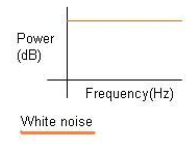
\includegraphics[scale=0.45]{images/I/wn.png}
  \caption{White noise}\label{fig:wn}
\end{figure}

\item[coloured noise]Colored noise will have different integrated power at different frequency bands of same duration. Depending upon whether it is gray, pink, blue or brown color it will have different power spectrum. Based on this power concentration varies at different frequencies. The figure describes spectrum of colored noise(example-Pink noise).
\begin{figure}[h!]
  \centering
  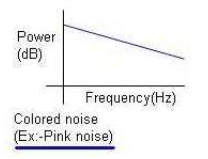
\includegraphics[scale=0.45]{images/I/cn.png}
  \caption{Coloured noise}\label{fig:cn}
\end{figure}


\item[Husid Plot] A plot of the build-up of Arias intensity with
time is known as a Husid plot (Figure 6) and it serves
to identify the interval over which the majority of
the energy is imparted. The root-mean-square acceleration (arms) is the equivalent constant level of
acceleration over any specified interval of the accelerogram; the arms is also the square root of the gradient of the Husid plot over the same interval. Arias
intensity has been found to be a useful parameter to
define thresholds of shaking that trigger landslides.
\begin{figure}[h!]
  \centering
  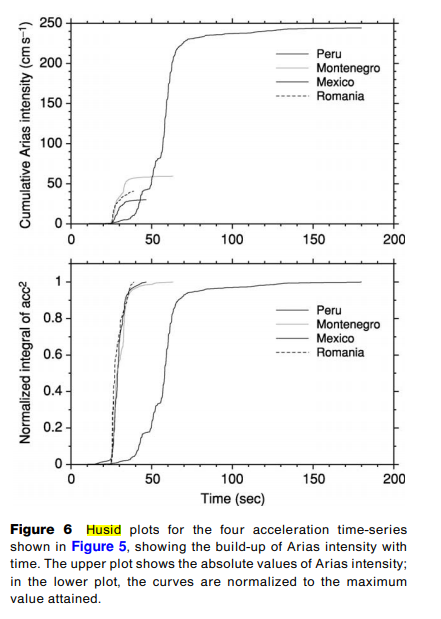
\includegraphics[scale=0.45]{images/I/husid.png}
  \caption{Husid Plot}\label{fig:husid}
\end{figure}
\end{itemize}


	
%---------------------------------------------------------------------------------------------------
%	BIBLIOGRAFIA
% bibliografia in formato bibtex
%	\backmatter
	\newpage\null\thispagestyle{empty}\newpage
    \bibliographystyle{siam}
	\nocite{*}    
    \bibliography{biblio}
% 	\addcontentsline{toc}{chapter}{Bibliografia}
%   
%---------------------------------------------------------------------------------------------------
% %	APPENDICI    

% % \input{Vuoto/Vuoto} 
% \thispagestyle{empty}
%   \addcontentsline{toc}{chapter}{Appendix}
%   \appendix
%   \newpage
\thispagestyle{myheadings}
\chapter[Appendix A - EC8 Spectrum]{- \hspace{0.5cm} Appendix}
\section*{\LARGE{EC8-Spectrum}}
\vspace{0.5cm}
\markboth{\MakeUppercase{Appendix A}}{\MakeUppercase{EC8-Spectrum}}
\label{app:spectra}


Script \ml~ to launch.
\begin{itemize}
    \item \verb|MAIN _ GLOBAL|
    \item input source 
            \begin{itemize}
                \item loading seismic input by preparing a .m array file (groupaccREVmajor.m);
                \item for each of the input file, the routine creates a folder inside which it collocates \verb|acc|, \verb|t|, \verb|dt|, \verb|name| and it is already converted in \verb|comma| files for SAP2000;
                \item it is also prepared both time histories and spectra graphics representation and arias intensity cuttings;
            \end{itemize}
    \item \verb|main_for_SAP(no_gms)|
            \begin{itemize}
                \item \verb|list_SAP_input_files| to know how many simulations will be runned;
                \item \verb|originalFile| prepare the .$2k$ file of SAP2000
                Pay attention that I missed the lines:
                TABLE:  TABLES AUTOMATICALLY SAVED AFTER ANALYSIS
                            SaveFile=Yes   FileName=output - from - SAP.xml   NamedSet=OUT-STRUCT-ALL   Group=ALL
                        END TABLE DATA
                        I prepare this file by opening reference file in SAP by the procedure: Define Database Table Set Names , select all flags.
                        \item \verb|label_set_to_change| what I should change inside the SAP file, so preparing it for the next regular expressions.
                        Therefore, I have tableset called labelName that collects all the info I will need to change during the analysis.
                        
            \end{itemize}
    
\end{itemize}
    
    
    
    \lstset{language=Tex,numbers=none}
       \begin{lstlisting}[frame=lines]

       \end{lstlisting}
%   \newpage
\thispagestyle{myheadings}
\chapter[Appendix B - Spectra-compatible Accelerogram]{- \hspace{0.5cm} Appendix}
\section*{\LARGE{Spectra-compatible Accelerogram}}
\vspace{0.5cm}
\markboth{\MakeUppercase{Appendix B}}{\MakeUppercase{Spectra-compatible Accelerogram}}
\label{app:B}

    \lstset{language=Tex,numbers=none}
       \begin{lstlisting}[frame=lines]
         Time history matched to spectrum:E:\Program Files(x86)\...
         ... GeoMotions\Output\RspMatch\EC08.tgt 
	PTS:4768      STEP:0.0050    
   0.24118E-04   0.24414E-04   0.24710E-04   0.25006E-04   0.25303E-04

       \end{lstlisting}

\end{document}
